\section{R2: Causal Profiling for Scale-out Architectures}
\label{sec:causalprofile}

\begin{figure}[!t]
  \centering
  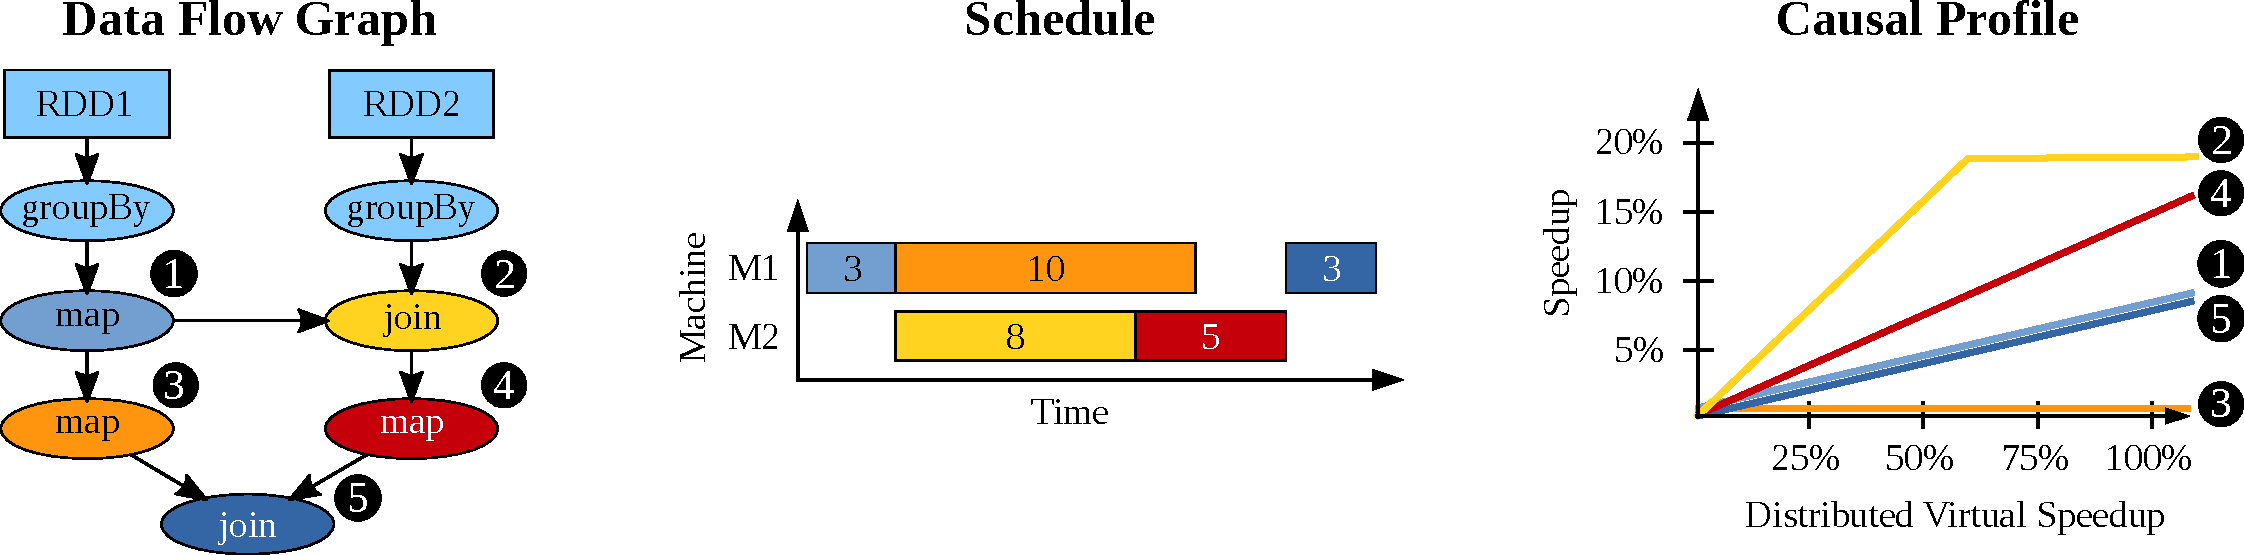
\includegraphics[width=0.90\textwidth]{fig/causal-prof2}
  \caption{
    Overview of causal profiling.
    The data flow graph represents a part of the Alternating Least
    Squares (ALS) algorithm~\cite{meng:sparkml}, about 1400 lines of
    code. At runtime, it consists of more than 1200 tasks.
    A schedule for the execution of the data flow graph for
    two machines is given along with the execution times for each
    task. The causal profile predicts the overall speedup based on
    speeding up the individual components, using both the data flow
    graph and the schedule as inputs. For example, it shows that
    optimizing task (2) is the most impactful one, whereas optimizing the
    longest running task (3) does not affect the overall runtime.
}
\label{f:causal-overview}
\vspace{-5px}
\end{figure}

Scale-out architectures are the standard and common approach to scale
applications in this cloud computing era.
For example, a distributed application in Google runs
on hundreds to a few hundred thousand machines~\cite{google:web} to
achieve high total computing power. At the same time,
finding performance bottlenecks in distributed applications is
notoriously difficult~\cite{pivot-tracing:sosp15, x-ray:osdi12,
  aguilera:dist-system-blackboxes, dist-debugging:queue16,
  whodunit:eurosys07, pinpoint:dsn02, fay:sosp11, x-trace:nsdi07,
  mtracer:sose14, lprof:osdi14, dapper:google10, flowdiff:nsdi11}.
There are a few reasons for such difficulty:
A distributed application is composed of many sub-tasks running on
different nodes.
The complex dependencies and interactions among sub-tasks impose difficulty
in pinpointing the performance bottlenecks.
As a result, optimizing a sub-task does not necessarily translate to an
improvement of the end-to-end performance.
For example, \autoref{f:causal-overview}
illustrate one such instance.
Counterintuitively, optimizing the (longest) sub-task
(3)
does not help to improve overall performance
because there is a dependency with a sub-task (5).
In addition, many other things can affect the overall
performance but are hard to predict: scheduling/straggler policies of
a distributed framework (e.g., Hadoop and Spark~\cite{zaharia:rdd}),
bottleneck on disk and network, and limping machines.

To tackle profiling of distributed applications, existing cluster
profilers employ a similar, yet distributed, approach to single-machine
profilers~\cite{spark:web, cluster:web} or find a critical path from
the execution graph constructed from logs~\cite{yang:critical-path,
aguilera:dist-system-blackboxes}.
However, neither is effective in
finding performance bottlenecks and predicting the potential improvement as an
optimization to improve end-to-end performance.
The former shows accumulated CPU usage per sub-task, but
as \autoref{f:causal-overview} shows, optimizing the most
CPU-consuming sub-task does not always improve performance.
The latter, finding a critical path, gives more information 
but does not provide any performance boundness guarantee of the optimization.
With such limited profiling results, developers
could waste their efforts optimizing a sub-task, which does not
affect the overall performance (i.e., ill-targeted optimization), or
its impact is marginal (i.e., diminishing returns or gold plating).

\boxbeg
\begin{Challenge}
  What is the optimal approach to identify optimization candidates in
  scale-out architectures that have high overall performance impact,
  considering myriad factors such as cluster scheduling and straggler
  mitigation?
\end{Challenge}
\boxend

In this research thrust, we will develop {\em causal profiling}
methods to identify performance bottlenecks in a distributed
application. In particular, we will estimate the impact of
optimizing a sub-task that will allow developers to choose the correct
optimization targets and stop the optimization before diminishing
returns begin to set in. \autoref{f:causal-overview} illustrates an
example of the distributed causal profiling. The causal profiler operates
on a data-flow graph induced by a distributed framework.
We will estimate the impact of optimization of
a sub-task on the overall performance using the {\em distributed virtual
speedup}; as the name suggests, it is an extension of
virtual speedup~\cite{curtsinger:coz} for distributed
applications (\autoref{sub:virtspeedup}). To find optimization
candidates without exhaustively running all possible candidates, we will
explore effective search space reduction techniques
(\autoref{sub:statereduction}). Finally, we will suggest optimization
candidates to developers (\autoref{sub:suggest}). We expect that some
of the techniques developed in this research will be applicable to
host-accelerator architectures, where accelerators (e.g., GPGPU, Intel
Xeon Phi, and FPGA) can act as remote nodes.


\subsection{R2.1 Emulating the Speedup of Distributed Tasks}
\label{sub:virtspeedup}
The {\em distributed virtual speedup} will predict the overall performance
impact of optimizing a task in a distributed application.
As speeding up any given code is not possible, we instead slow down all other
code by a given percentage while letting the original code run at full
speed.
This will estimate the impact of an optimization by the given percentage of the
task. For example, to estimate the impact of 10\% optimization
on a given method, we will slow down all other methods by 10\% while
running the given method at the original speed.

\boxbeg
\begin{Challenge}
  How can we extend the virtual speed to distributed applications
  (i.e., distribute virtual speedup) without modifying existing source
  code?
\end{Challenge}
\boxend

We plan to intercept the remote procedure call (RPC) layer.
Distributed frameworks, such as Hadoop or Spark, rely on RPC to
transparently execute remote tasks. We will intercept RPC messages and
selectively delay the delivery of messages that should be slowed
down for the distributed virtual speedup. To intercept messages and
delay their delivery without modifying source code, we will explore
dynamic reflection mechanisms (e.g.,
AspectJ~\cite{aspectj-introduction, aspectj:ecoop01}).


\subsection{R2.2 Effective Exploration of Search Space}
\label{sub:statereduction}
\boxbeg
\begin{Challenge}
Any non-trivial distributed application comprises a large
number of procedures. Furthermore, a single procedure can execute on
hundreds or thousands of machines. Thus, the search space of the
distributed virtual speedup is huge (e.g., product of the number of
procedures and the number of machines).
Thus, an important question is how to reduce the number of
possible combinations to quickly finish the analysis in a cost-effective
manner and generate a sufficient profile in a cloud environment?
%To finish an analysis quickly
%and in a cost-efficient manner when running in a cloud environment
%(e.g., Amazon EC2), it is imperative to reduce the number of possible
%combinations that need to be explored for a sufficient profile.
\end{Challenge}
\boxend

To effectively find optimization candidates without exhaustively
exploring all combinations of the distributed speed up, we will
use a {\em feedback-driven sampling approach}, where the next sub-task
for the distributed virtual speedup will be stochastically decided
based on the results of previous runs and guiding
heuristics. We will explore the search space in three steps:
%
First, we will exploit the execution structure of a distributed
applications For example, Spark operates on data-flow graphs that can
be expressed as directed acyclic graphs (DAG) comprising
sub-tasks. We can choose the probable sub-tasks for a speedup and can
bias the sampling toward these candidates; probable sub-tasks could be
sub-tasks on a critical path, or pre-/post-dominators of a join point.
%
Second, as previous research~\cite{altman:oopsla10} shows, there are
similarities in performance bottlenecks even among different
applications; we plan to explore machine learning techniques on
previously found bottlenecks to prune the search space.
%
Finally, we will incorporate the developers' knowledge to further
reduce the search space. Developers can suggest procedures to the
causal profiler that may or may not yield a positive effect
on the application while reducing the number of procedures to explore.


\subsection{R2.3 Suggesting Optimization Candidates}
\label{sub:suggest}
The output of the distributed causal profiler is a set of graphs that
quantify the distributed virtual speedup over the real speedup of
the application. This graph will be compiled from the data gathered
over multiple runs of the system, using different combinations of
distributed virtual speedups and the procedure to be sped up.

\boxbeg
\begin{Challenge}
  From the potentially large set of profiles, we need to prioritize
  distributed virtual speedup results in the order of possible speedup
  that will allow developers tackle the most plausible optimization
  candidates first.
\end{Challenge}
\boxend

We will experiment with various metrics to prioritize candidates. For
example, we suggest ones with the highest possible speedup for the
greatest performance improvement by optimizing a procedure; we suggest ones
with the steepest speedup curve to find low hanging fruits. In addition,
we consider the length of the code segment that was profiled, with
shorter segments being given higher preference, as these code segments
promise to be easier targets for optimization.
